%==============================
\section{Problem Formulation}\label{sec:problem}

%==============================
\begin{figure*}[t!]
	\centering
	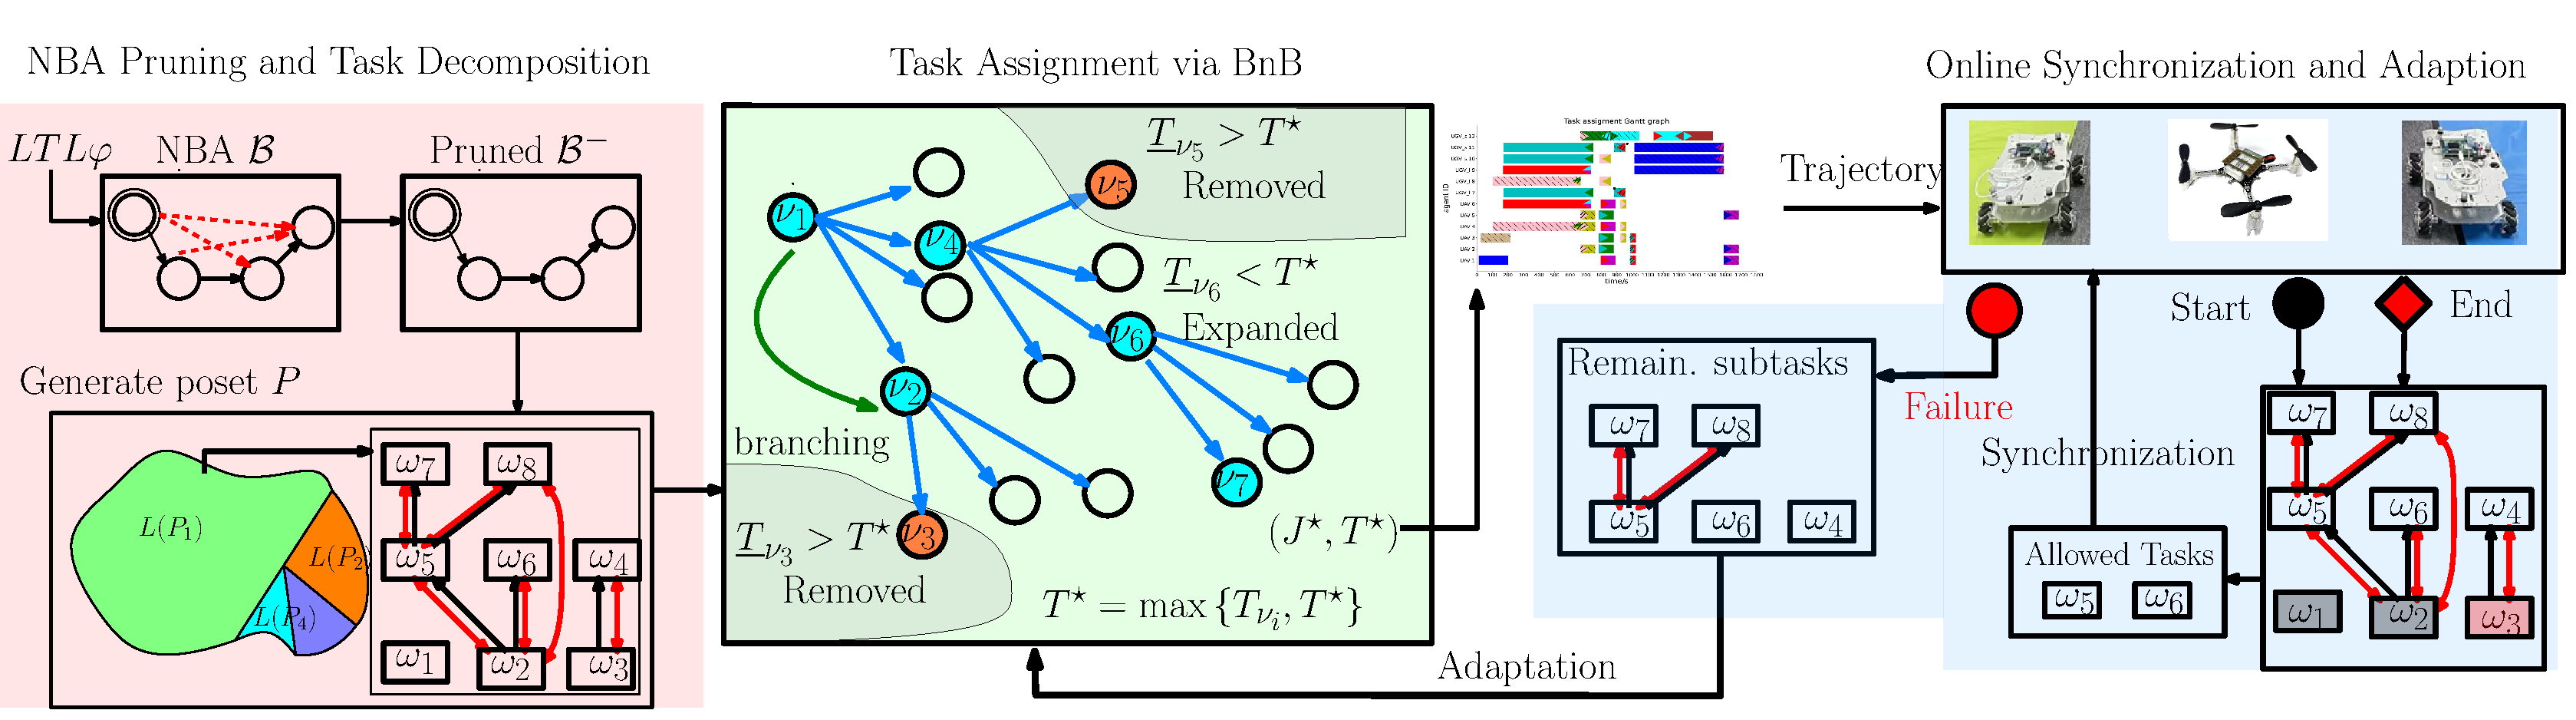
\includegraphics[width=0.9\linewidth]{figures/logic_fig1.pdf}
	%--------------------
	\caption{Overall structure of the proposed framework,
          which consists of three main parts:
        the computation of the posets, BnB search, and online execution.}
	\label{fig:logic_graph}
	%--------------------
\end{figure*}
%==============================

%==============================
\subsection{Collaborative Multi-agent Systems}\label{subsec:multi-agent}

Consider a team of $N$ agents operating in a workspace as~${W}\subset \mathbb{R}^3$.
Within the workspace, there are $M$ regions of interest,
denoted by ${\mathcal{W}}\triangleq \{{W}_1,{W}_2,\,\cdots,{W}_M\}$, 
where~${W}_m\in {W}$.
Each agent~$n\in\mathcal{N}=\{1,\cdots,N\}$ can navigate within these regions
following its own transition graph, i.e., $\mathcal{G}_n=({\mathcal{W}},\,\rightarrow_n,\,d_n)$,
where $\rightarrow_n\subseteq {\mathcal{W}}\times {\mathcal{W}}$
is the allowed transition for agent~$n$;
and $d_n:\rightarrow_n \rightarrow \mathbb{R}_{+}$ maps each transition to its time duration.

Moreover, similar to the action model used in our previous work~\cite{guo2016task},
each robot $n\in \mathcal{N}$ is capable of performing a set of actions:
$\mathcal{A}_n\triangleq \mathcal{A}^{\texttt{l}}_n \cup \mathcal{A}^{\texttt{c}}_n$,
where $\mathcal{A}^{\texttt{l}}_n$ is a set of \emph{local} actions that can be independently performed by agent $n$ itself;
$\mathcal{A}^{\texttt{c}}_n$ is a set of \emph{collaborative} actions that can only be performed
in collaboration with other agents.
Moreover, denote by~$\mathcal{A}^c\triangleq\bigcup_{n\in\mathcal{N}}\mathcal{A}^c_n$,
$\mathcal{A}^l\triangleq\bigcup_{n\in\mathcal{N}}\mathcal{A}^l_n$.
More specifically,
there is a set of collaborative behaviors pre-designed for the team,
denoted by~$\mathcal{C}\triangleq \{C_1,\cdots, C_K\}$. 
Each behavior $C_k\in \mathcal{C}$ consists of a set of collaborative actions
that should be accomplished by different agents, namely:
\begin{equation}\label{eq:c-k}
C_k\triangleq \{a_1,\,a_2,\cdots,a_{\ell_k}\},
\end{equation}
where~$\ell_k>0$ is the number of collaborative actions required;
~$a_{\ell}\in \mathcal{A}^c$, $\forall \ell=1,\cdots,\ell_k$.
Thus, each collaborative action has a fixed duration as~$d:\mathcal{C}\rightarrow \mathbb{R}_{+}$.
For instance, formation~\cite{chen2005formation}, herding~\cite{pan2007multi},
 consensus~\cite{li2009consensus} and coverage~\cite{mesbahi2010graph}
 are common collaborative behaviors of multi-agent systems.



%====================
\begin{remark}\label{rm:collaborative}
Different from~\cite{luo2021temporal,sahin2019multirobot, jones2019scratchs},
the definition of collaborative behavior above does not specify explicitly
the agent identities or {types}, rather their capabilities.
This subtle difference can improve the flexibility of the underlying solution,
e.g.,  no hard-coding of the agent identities or types is necessary;
any capable agent can be recruited for the collaborative behavior.
\hfill $\blacksquare$
\end{remark}
%====================



%==============================
\subsection{Task Specification}\label{subsec:task-specification}
First, the following three types of atomic propositions can be introduced:
(i) $p_m$ is \emph{true} when \emph{any} agent $n\in \mathcal{N}$ is at region ${W}_m\in {\mathcal{W}}$;
Let $\mathbf{p}\triangleq \{p_m,\, \forall {W}_m \in {\mathcal{W}}\}$;
(ii) $a^m_k$ is \emph{true} when a \emph{local} action~$a_k$ is performed at region ${W}_m\in{\mathcal{W}}$ by
agent~$n$, where $a_k \in \mathcal{A}_n^{\texttt{l}}$.
Let~$\mathbf{a} \triangleq\{a^m_k,\forall {W}_m \in \mathcal{W}, a_k\in \mathcal{A}^{l}\}$;
(iii) $c^m_k$ is \emph{true} when the collaborative behavior~$C_k$ in~\eqref{eq:c-k} is performed at region $W_m$.
Let $\mathbf{c} \triangleq\{c^m_k,\forall C_k \in \mathcal{C},\forall {W}_m \in {\mathcal{W}}\}$.

Given these propositions, a team-wide task specification can be specified as a sc-LTL formula
\begin{equation}\label{eq:task}
\varphi=\textup{sc-LTL}(\{\mathbf{p}, \mathbf{a}, \mathbf{c}\}),
\end{equation}
where the syntax of sc-LTL is introduced in Sec.~\ref{subsec:LTL}.
Denote by~$t_0,\, t_f>0$ the time instants when the system starts
and satisfies executing~$\varphi$, respectively.
Thus, the total time taken for the multi-agent team to satisfy~$\varphi$ is given by:
\begin{equation}\label{eq:task-freq}
T_\varphi = t_f-t_0.
\end{equation}
Since a sc-LTL can be satisfied in finite time, this total duration is finite and thus can be optimized. 


%====================
\begin{remark}\label{rm:cost}
  As described previously in Sec.~\ref{sec:introduction}, the minimum time cost in~\eqref{eq:task-freq} is significantly different from the summed time cost of all agents, i.e.,
$\sum_{i} T_i$, where~$T_i$ is the total time agent~$i$ spent on executing task~$\varphi$,
as in~\cite{kantaros2020stylus, schillinger2018simultaneous, guo2016task, luo2021temporal}.
The main advantage of concurrent execution can be amplified via
the objective of time minimization,
since concurrent or sequential execution of the same task assignment could
be equivalent in terms of summed cost.
\hfill $\blacksquare$
\end{remark}
%====================
\begin{example}\label{exp:task}
Consider a team of UAVs and UGVs deployed for maintaining a remote Photovoltaic power plant.
One collaborative task considered in Sec.~\ref{sec:experiments} is given by:
\begin{equation}\footnotesize
\label{example:task} 
\begin{aligned}
\varphi_1 = & \Diamond(\texttt{repair}_{\texttt{p}_{3}} \wedge \lnot \texttt{scan}_{\texttt{p}_3} \wedge\Diamond \texttt{scan}_{\texttt{p}_3})
\wedge \Diamond (\texttt{wash}_{\texttt{p}_{21}} \wedge \\
&\Diamond \texttt{mow}_{\texttt{p}_{21}} \wedge \Diamond \texttt{scan}_{\texttt{p}_{21}}) \wedge \Diamond ( \texttt{sweep}_{\texttt{p}_{21}} \wedge \lnot \texttt{wash}_{\texttt{p}_{21}} \wedge\\
& \Diamond \texttt{mow}_{\texttt{p}_{21}}) \wedge \Diamond(\texttt{fix}_{\texttt{t}_5} \wedge \lnot \texttt{p}_{\texttt{18}}) \wedge \lnot \texttt{p}_{24} \,U \, \texttt{sweep}_{\texttt{p}_{27}} \\
&\wedge \Diamond (\texttt{wash}_{\texttt{p}_{34}} \wedge \bigcirc \texttt{scan}_{\texttt{p}_{34}}),
\end{aligned}
\end{equation}
which means to repair and scan certain PV panel $p_3$
in a given order, deeply cleaning the panel $p_{21},p_{34}$, fix transformers
$t_5$, sweep $p_{27}$ with safety request. 
 \hfill $\blacksquare$
\end{example}
%==============================
\subsection{Problem Statement}\label{subsec:problem-statement}

\begin{problem}\label{prob:formulation}
Given the task specification~$\varphi$,
synthesize the motion and action
sequence for each agent $n\in \mathcal{N}$,
such that~$T_{\varphi}$ in~\eqref{eq:task-freq} is minimized.
\hfill $\blacksquare$
\end{problem}
Even through the above problem formulation is straightforward,
it is can be shown that this problem belongs to the class of NP-hard
problems~\cite{hochba1997approximation, bovet1994introduction},
as its core coincides with the makespan minimization problem
of flow-shop scheduling problems.
Various approximate algorithms have been proposed in~\cite{khamis2015multi, hoos2004stochastic}.
However,
the combination of dynamic vehicles within a graph-like environment,
linear temporal constraints,
and collaborative tasks has not been addressed.
